\documentclass{beamer}
\mode<presentation>
\usetheme{Madrid}
\usecolortheme{crane}

\usepackage{tikz}
\usepackage{epic}
\usepackage{qtree}
\usepackage{linguex}
\usepackage[normalem]{ulem}
\usepackage{tikz-dependency}
\usepackage{colortbl}
\usepackage{xcolor}
\definecolor{darkgreen}{rgb}{0,0.3,0}
\definecolor{darkblue}{rgb}{.05,.05,.30}
\definecolor{lightgrey}{rgb}{0.65,0.65,0.65}
\definecolor{darkred}{rgb}{0.4,0,0}
\usepackage{tikzsymbols}
\usepackage{amsmath}
\usepackage{multirow}
\usepackage{setspace}
\usepackage{verbatim}

\newcommand{\norm}[1]{\left\lVert#1\right\rVert}
\newcommand{\remph}[1]{\textbf{\color{red} #1}}
\newcommand{\argmax}{\arg\max}

\makeatletter
\newcommand{\xRightarrow}[2][]{\ext@arrow 0359\Rightarrowfill@{#1}{#2}}
\makeatother
\usetikzlibrary{calc}
\usetikzlibrary{matrix,arrows,positioning,automata,shadows,shapes.geometric}

\title[LT2222 lecture 5]{LT2222 Machine learning for statistical NLP: intro, Winter 2021}
\subtitle{Lecture 5: perplexity; backpropagation}
\author[Sayeed]{Asad Sayeed\\{\tiny with material adapted from {\tt https://github.com/jonsafari/lt1}}}
\institute[Gothenburg]{University of Gothenburg}
\date{}

\setbeamertemplate{navigation symbols}{}

\newcommand{\placard}[1]{
  \begin{frame}
    \begin{center}
      \huge
      \textbf{#1}
    \end{center}
  \end{frame}
}

\newcommand{\pagestep}[2]{
  \begin{frame}[t]
    \begin{minipage}[t][0.26\textheight][t]{\textwidth}
      \begin{center}
        \huge
        \textbf{#1}
      \end{center}
    \end{minipage}
    
    \begin{minipage}[t][0.7\textheight][c]{\textwidth}
      \begin{center}
        \includegraphics[height=0.83\textheight]{#2}
      \end{center}
    \end{minipage}
  \end{frame}
}

\newcommand{\pagestepalt}[2]{
  \begin{frame}[t]
    \begin{minipage}[t][0.26\textheight][t]{\textwidth}
      \begin{center}
        \huge
        \textbf{#1}
      \end{center}
    \end{minipage}
    
    \begin{minipage}[t][0.7\textheight][c]{\textwidth}
      #2
    \end{minipage}
  \end{frame}
}

\newcommand{\pagestepaltf}[2]{
  \begin{frame}[fragile]
    \begin{minipage}[t][0.26\textheight][t]{\textwidth}
      \begin{center}
        \huge
        \textbf{#1}
      \end{center}
    \end{minipage}
    
    \begin{minipage}[t][0.7\textheight][c]{\textwidth}
      #2
    \end{minipage}
  \end{frame}
}


%% \newcommand{\pagestepaltfragile}[2]{
%%   \begin{frame}[fragile][t]
%%     \begin{minipage}[t][0.26\textheight][t]{\textwidth}
%%       \begin{center}
%%         \huge
%%         \textbf{#1}
%%       \end{center}
%%     \end{minipage}
    
%%     \begin{minipage}[t][0.7\textheight][c]{\textwidth}
%%       #2
%%     \end{minipage}
%%   \end{frame}
%% }


\begin{document}
\makeatletter
\setbeamertemplate{footline}
{
  \leavevmode%
  \hbox{%
  \begin{beamercolorbox}[wd=.333333\paperwidth,ht=2.25ex,dp=1ex,center]{author in head/foot}%
    \usebeamerfont{author in head/foot}\insertshortauthor\expandafter\beamer@ifempty\expandafter{\beamer@shortinstitute}{}{~~(\insertshortinstitute)}
  \end{beamercolorbox}%
  \begin{beamercolorbox}[wd=.333333\paperwidth,ht=2.25ex,dp=1ex,center]{title in head/foot}%
    \usebeamerfont{title in head/foot}\insertshorttitle
  \end{beamercolorbox}%
  \begin{beamercolorbox}[wd=.333333\paperwidth,ht=2.25ex,dp=1ex,right]{date in head/foot}%
    \usebeamerfont{date in head/foot}\insertshortdate{}\hspace*{2em}
%    \insertframenumber{} / \inserttotalframenumber\hspace*{2ex} 
    \insertframenumber{}\hspace*{2ex}
    \hspace*{6ex}
  \end{beamercolorbox}}%
  \vskip0pt%
}
\makeatother


\begin{frame}
  \titlepage
\end{frame}


\pagestepalt{Today's agenda:}{
  \begin{enumerate}
  \item Perplexity
  \item Backpropagation
  \end{enumerate}
}

\placard{Part 1: Perplexity}

\pagestepalt{What is perplexity?}{
  From Wikipedia:
  \begin{block}{Perplexity}
    Perplexity is a measure of how well a probability distribution predicts a sample\ldots A low perplexity indicates the probability
    distribution is good at predicting the sample.
  \end{block}\pause
  If you are trying to test a distribution, it's just:
  \[
  2^{H(p)} = 2^{-\sum_x p(x) \log_2 p(x)}
  \]
  i.e., the sum over all possible events $x \in X$ of the entropy.\\ \pause
  Intuitively, it's about how ``hard'' it is for the probability distribution to make binary ``decisions''.
}

\pagestepalt{Perplexity of a model}{
  When you are trying to measure the difficulty of a \alert{model} in ``deciding'' a sample:\pause
  \[
  2^{-\frac{1}{N} \sum_N^{i=1} \log_2 q(x_i)}
  \]
  where $q$ represents the model probabilities and $N$ is the number of samples.\pause\\
  What happened to $p$?\pause
  \begin{itemize}
  \item $p$ is the unknown sample distribution.\pause
  \item Consider that each event (word) $x$ has a probability $\frac{n}{N}$ if $x$ occurred $n$ times in the test corpus. Since there are a total of $N$ occurrences of all words, we can factor this out and take the average with $\frac{1}{N}$\pause
  \item (You are now measuring ``decisions'' in terms of the cross-entropy between ``empirical'' $p$ and model $q$.)
  \end{itemize}
}

\pagestepalt{Perplexity of a language model}{
  It's just model perplexity based on the average log probability of each word\ldots
  \begin{itemize}
  \item You just compute it over each word by applying your model.\pause
  \item The lower perplexity the better.\pause
  \item Perplexities are not comparable between texts, they measure the predictive power of different models \alert{given} a test corpus.
  \end{itemize}
}

\placard{Part 2: Backpropagation}

\pagestepalt{Brief interlude}{
\begin{description}
\item[Hadamard Product]: Multiplying corresponding elements of two vectors\pause. Also called \textit{element-wise product}
	\begin{align*}
		{\bf x \odot y} &= {\color{gray}{\bf x \circ y}} = \langle x_1 \, y_1, \ x_2 \, y_2, \ x_3 \, y_3, \ \ldots \rangle \\[0.5em]
					&= \langle (2.1 \times 1.1), (-8.5 \times 5.0), (0.1 \times -4.4) \rangle \\
					&= \langle 2.31, -42.5, -0.44 \rangle
	\end{align*}
%	\code{x * y}
\end{description}
}

\placard{Previously we talked about gradient descent\ldots}

\pagestepalt{Zig-zag}{
  The gradient descent algorithm does not go
  ``cleanly'' down the gradient (Wikipedia again).
  \vspace{-0.5cm}
  \begin{columns}[T]
    \begin{column}{0.49\textwidth}
      \begin{center}
        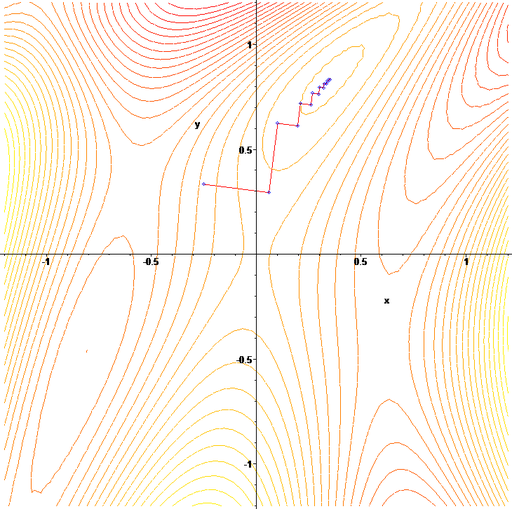
\includegraphics[width=0.9\textwidth]{grad1.png}
      \end{center}
    \end{column}
    \begin{column}{0.49\textwidth}
      \begin{center}
        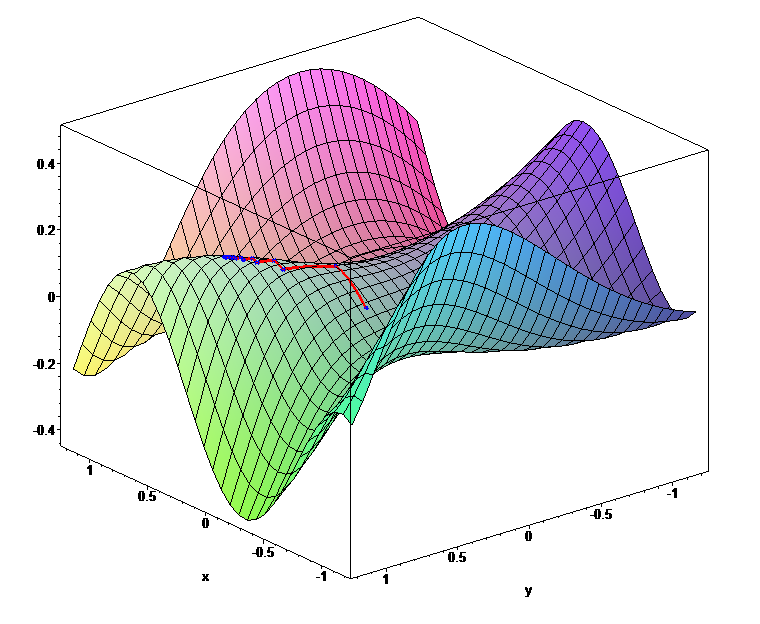
\includegraphics[width=0.9\textwidth]{grad2.png}
      \end{center}
    \end{column}
  \end{columns}
}


\pagestepalt{Stochastic gradient descent\ldots}{
  \ldots looks like this:
  \begin{block}{(Wikipedia says\ldots though I changed the variable names)}
    \begin{enumerate}
    \item Choose an initial vector of parameters $\mathbf{w}$ and a learning rate $\gamma$.
    \item Repeat until an approximate minimum is obtained.
      \begin{itemize}
      \item Randomly shuffle the examples in the training set.
      \item For $i = 1,2,\ldots,n$ do:
        \begin{itemize}
          \item $\mathbf{w} \Leftarrow \mathbf{w} - \gamma\nabla F_i(\mathbf{w})$
        \end{itemize}
      \end{itemize}
    \end{enumerate}
  \end{block}
  \begin{itemize}
  \item Can pick a ``mini-batch'' instead of instance-by-instance.
    \begin{itemize}
    \item So need to choose learning rate and batch size.
    \end{itemize}
  \item Convergence -- not exactly guaranteed, but very likely.
  \end{itemize}
}

\placard{Problem: how do we operationalize this over neurons?}

\pagestepalt{Backpropagation from loss}{
  Propagation phase:\pause
  \begin{enumerate}
  \item \alert{Propagate forward}: feed the input (training
    example) through the network until we get values at the output layer.\pause
  \item \alert{Compute error/cost}: that is, apply the loss function to the output values.\pause
  \item \alert{Propagate backwards} (duh!): Calculate differences between output and expected values
    for output layer and hidden layers (the ``output delta'' $\delta$).\pause
    \begin{itemize}
    \item This is the ``miracle'' part.
    \item We have to distribute the cost at each node to each of the nodes at the previous layer.
    \end{itemize}
  \end{enumerate}
  Then we need the weight update\ldots
}

\pagestepalt{Backpropagation from loss}{
  Weight update phase (this is the mathy part). For each node:\pause
  \begin{enumerate}
  \item Find the gradient of the weight (this is how we operationalize $\nabla F$!):
    multiply the output delta $\delta$ with the input activation.\pause
  \item The multiply the learning rate $\gamma$ (as a percentage) of
    the gradient with $\delta$ and subtract it from the node's weight.\pause
  \end{enumerate}
  And you keep doing this at every batch, for every node. This is how
  we implement the gradient descent formula\\
  \[\mathbf{w} \Leftarrow \mathbf{w} - \gamma\nabla F_i(\mathbf{w})\]
}

\pagestepalt{In equations}{
  \vspace{-1.0cm}
  But we conceive of this in terms of
  vectors rather than individual nodes, because it's faster.\pause
  \begin{itemize}
  \item  Say $\mathbf{z}^L$ is the vector representing the output of the output layer.
    Then $\mathbf{\delta}^L$ is given by:
    \begin{block}{}
      \[\mathbf{\delta}^L = \nabla F \odot \sigma'(\mathbf{z}^L)\]
    \end{block}
    where $\sigma'$ represents the measured rate of change in the output values.\pause
  \item Then we can recurrently compute the error in any layer $\mathbf{\delta}^l$
    \begin{block}{}
      \[\delta^l = ((\mathbf{W}^{l+1})^T \mathbf{\delta}^{l+1}) \odot \sigma'(\mathbf{z}^l))\]
    \end{block}
    where $\mathbf{W}^{l+1}$ is the weight matrix at layer $l+1$. 
  \end{itemize}
}

\pagestepalt{Another miracle}{
  But then say that $\mathbf{a}^l$ is the \alert{activation} -- ie, the outputs coming ``in'' from the
  previous layer.\pause\\
  \begin{columns}
    \begin{column}{0.49\textwidth}
      The gradient we subtract from the weights changes, so we converge over time:
      \begin{block}{(Very loosely, for a given node $j$)}
        \[\gamma^l = \frac{\partial F}{\partial w^l_j} = {a}^{l-1}_k \delta^l\]
      \end{block}      
      Where $k$ are the incoming nodes.\pause\\
      That is, the weight update is
      variable based on the error.\pause
    \end{column}
    \begin{column}{0.49\textwidth}
      (from Sebastian Raschka on Quora, using different variable names)
      \begin{center}
        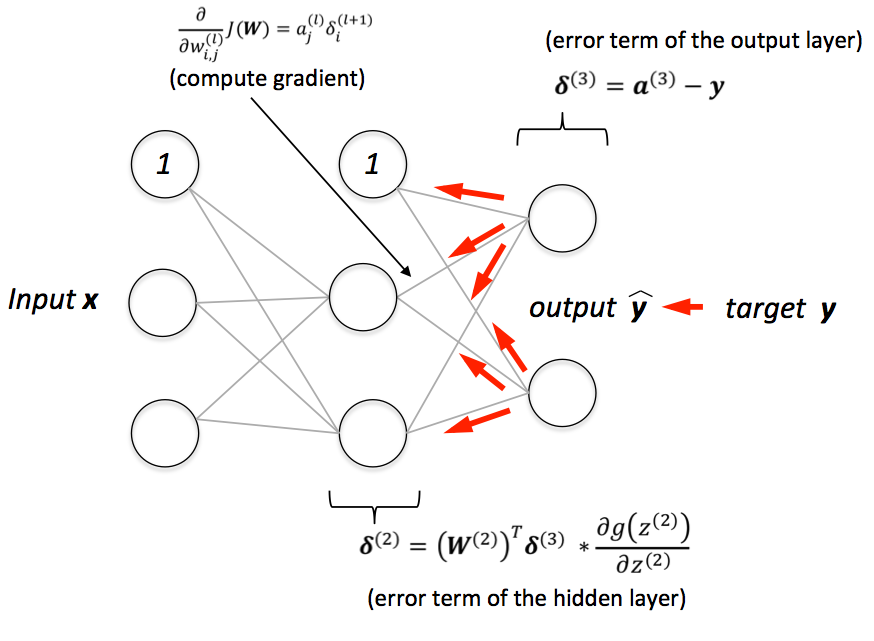
\includegraphics[width=0.8\textwidth]{backprop.png}
      \end{center}
    \end{column}
  \end{columns}
}

\end{document}
